\chapter{Introdução}
\label{c_introducao}

A depuração é entendida como um dos conceitos centrais do aprendizado de programação \cite{carver_assessing_1986}. Ela compreende a etapa de encontrar e solucionar problemas ou \textit{bugs}\footnote{
    Termo em inglês que, quando ligado à informática, significa falha ou defeito em código que provoca mau funcionamento.
} em algoritmos. \citeonline{mccauley_debugging_2008} menciona que a depuração é um tema de difícil aprendizado para os estudantes e um desafio de ensino para os professores. Neste sentido, a literatura sobre o tema busca responder questões como: quais as causas dos \textit{bugs}, quais categorias de \textit{bugs} são mais frequentes?, e como melhorar o ensino e aprendizado de depuração?

Enquanto no contexto comercial os erros em \textit{software} são indesejados e causam prejuízos de toda ordem \cite{valdivia-garcia_understanding_2016}, no campo educacional eles representam oportunidades de aprendizado. Segundo \citeonline{papert_mindstorms:_1980}, não se espera que qualquer coisa funcione na primeira tentativa, portanto errar e depurar faz parte do processo. 

\citeonline{valente_aspectos_2018} expressa essa ideia como uma espiral de \textit{descrição-execução-reflexão-depuração} (\autoref{fig_espiral}). Ao entrar nessa espiral, primeiramente o aluno descreve um programa e o executa, para obter um resultado. Pode, então, refletir sobre se a execução do seu programa resultou naquilo que intencionava. Por fim, em caso negativo, deve depurar o programa. Essa depuração pode eliminar erros de sintaxe, revelar incompreensão de conceitos envolvidos no problema ou esclarecer quais passos devem ser aplicados para resolvê-lo. Esse ciclo possibilita ao aluno passar de um nível de conhecimento inicial para outro mais elaborado.

\begin{figure}[!htpb]
  \centering
  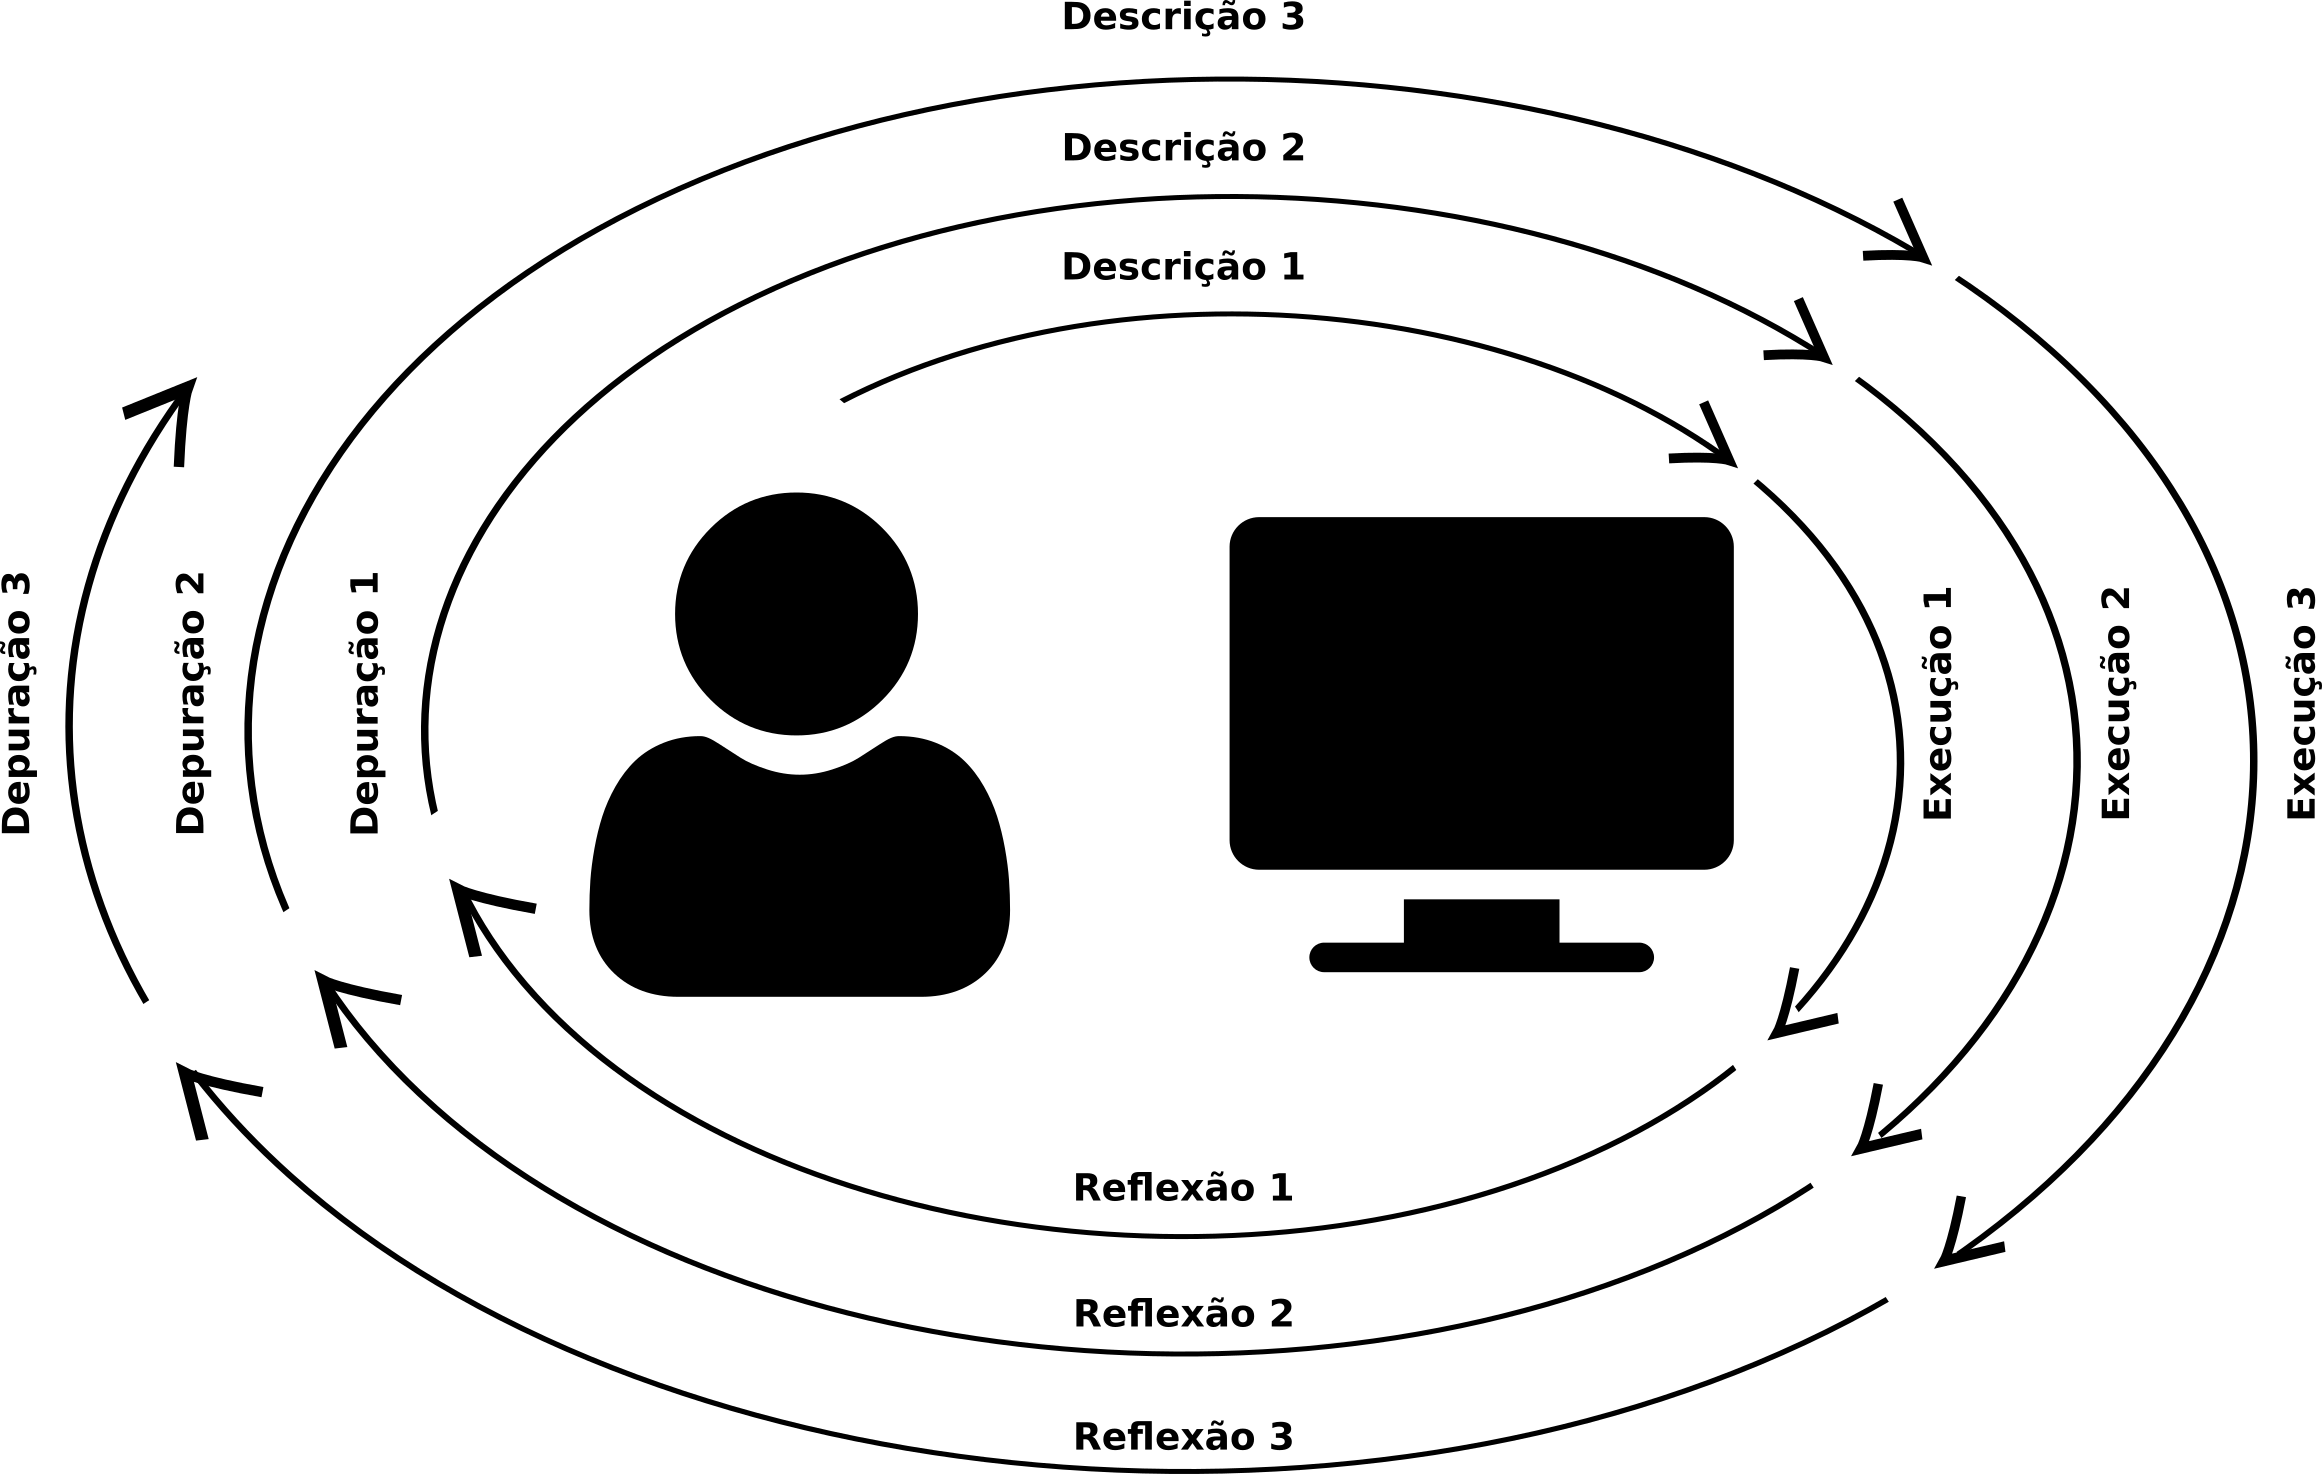
\includegraphics[width=.6\linewidth,fbox]{figs/ciclo_descricao_execucao_reflexao_depuracao.png}
  \caption{Espiral de aprendizagem.}
  \source{Adaptado de \citeonline{valente_aspectos_2018}.}
  \label{fig_espiral}
\end{figure}

A depuração também foi uma das diretrizes de design do ambiente de programação Logo \cite{solomon_history_2020}. Desenvolvido a partir de 1966, ele foi o primeiro ambiente de programação projetado para crianças. Era composto por um computador, uma linguagem textual de programação e um robô com rodas que se movia no chão e desenhava sobre papel. Esse ambiente permitia depurar por meio instruções da própria linguagem, como \textit{pause}, impressão de pilha de comandos e impressão de variáveis. 

Além desses recursos técnicos, para \citeonline{solomon_history_2020} a "grande ideia"\ do Logo era permitir à criança depurar seu próprio entendimento do processo computacional e do algoritmo a ser implementado. Um exemplo é o entendimento dos comandos \textit{left} e \textit{right}, que as crianças confundiam com mover para o lado. Para auxiliar a criança depurar esse conceito, um professor poderia sugeri-la "brincar de ser programada", para então compreender que esses comandos representam movimentos de giro.

A ideia de que a depuração poderia representar uma atividade benéfica para o desenvolvimento cognitivo, somada à existência da linguagem Logo, estimulou pesquisas sobre a prática de depuração por crianças. \citeonline{carver_assessing_1986} avaliaram a depuração de algoritmos por crianças de 7 a 8 anos durante um curso usando Logo. Para isso definiram um modelo de depuração em quatro fases: (i) identificação da diferença entre resultado esperado e resultado obtido; (ii) levantamento de hipóteses para a causa do erro; (iii) localização do \bug\ no código; e (iv) correção do \bug. Com base neste modelo, os pesquisadores concluíram que, após 24 horas de curso, as crianças não desenvolveram estratégias efetivas de depuração, preferindo apagar todo o código e escrever novamente. Posteriormente os mesmos autores conseguiram identificar que crianças aprenderam procurar erros e transferiram esta habilidade para atividades não relacionadas à programação \cite{carver_improving_1987}.

Além de possibilitar pesquisas sobre como as crianças programam, o ambiente Logo contribuiu para o surgimento, na década de 1990, de um ramo de estudos de \ac{IHC} focado no design de interação para crianças \cite{hourcade_child-computer_2015}. Esse ramo de estudos permitiu identificar dificuldades que as crianças tinham ao usar teclado de computadores convencionais \cite{mcnerney_turtles_2004}, projetados para adultos. O uso dos teclados exigia alfabetização, coordenação motora fina, e propiciava a ocorrência de erros sintáticos. Esses aspectos desviavam a atenção que deveria estar focada na construção de algoritmos e entendimento do problema para aspectos secundários, como entender o funcionamento da interface.

O reconhecimento dessa inadequação na interação das crianças com o ambiente de programação, motivou a criação de uma classe de ferramentas dos \ac{BPs}. Os \ac{BPs} descendem do ambiente Logo e buscam facilitar o aprendizado de programação pelo público infantil. Assim como o robô do ambiente Logo, eles geralmente se movem sobre o chão, e tem aparências que remetem ao imaginário infantil, como animais, carros ou robôs \cite{raabe_2017_rope}. Em geral, sua principal funcionalidade é possibilitar à criança inserir comandos, que o brinquedo então executa. Esses brinquedos têm interfaces de programação projetadas para facilitar à criança concentrar-se nos conceitos fundamentais, sem se distrair com erros que não contribuem para o aprendizado de algoritmos.

As interfaces dos \ac{BPs} são simplificadas, para que crianças pequenas saibam como interagir. Adicionar controles de depuração nessas interfaces aumenta a sua complexidade. Ambientes de desenvolvimento profissionais e/ou voltados para o ensino de programação introdutória para adultos apresentam controles de depuração. Esses ambientes mostram valores de variáveis, permitem executar passo a passo e definir pontos de parada \cite{noschang_portugol_2014}. Se adultos precisam destas ferramentas, será que as crianças poderiam se beneficiar das mesmas funcionalidades caso aplicadas em interfaces de \ac{BPs}?

 \citeonline{sipitakiat_robo-blocks_2012} tentam responder essa pergunta ao criar o Robo-Blocks, uma interface tangível de programação em blocos que permite execuções passo a passo. Os autores perceberam que as crianças implementavam “grosseiramente” suas ideias para ver o robô executá-las, sem refletir e aprender com os erros. Além disso, os movimentos rápidos do robô não permitiam comparar as ações do brinquedo com os blocos de “código”, dificultando associar um movimento errado com um bloco. Neste sentido, a execução passo a passo permitiu associar blocos com movimentos, o que foi auxiliado por um LED ativado em cada bloco durante sua execução. 
 
O Cubetto \cite{anzoategui_cubetto_2017} (\autoref{fig_cubetto}) é um \ac{BP} é programado por um painel onde são encaixados blocos de madeira. O painel destaca cada bloco executado acendendo LEDs. Permite, portanto, que a criança associe o movimento do brinquedo com sua causa na lista de comandos. Diferente do Robo-Blocks, porém, não há a opção de execução passo a passo. O Cubetto e o Robo-Blocks, portanto, tentam atacar o problema da depuração em interfaces que devem ser compreendidos por crianças.

Uma característica comum nestes trabalhos é a presença de componentes eletrônicos. Eles têm baterias, conectores e placas eletrônicas. Como alternativa, \citeonline{fincher_tangible_2019} apresentam as “linguagens externamente compiladas”. Elas são interfaces com blocos tangíveis que contém marcas especiais, denominadas marcas fiduciais. Essas marcas são lidas por um sensor óptico e interpretadas por um software que identifica as marcas e as converte em um conjunto de comandos para o brinquedo executar. Deste modo os blocos não carecem de componentes eletrônicos, aumentando a liberdade para os projetistas escolherem os materiais ou objetos a utilizar \citeonline{fincher_tangible_2019}. O KIBO \cite{sullivan_kibo_2015} (\autoref{fig_kibo}) é um executado de \ac{BP} programado por uma linguagem externamente compilada.

\begin{figure}[!htbp]
    \centering
    \begin{subfigure}{.5\textwidth}
        \centering
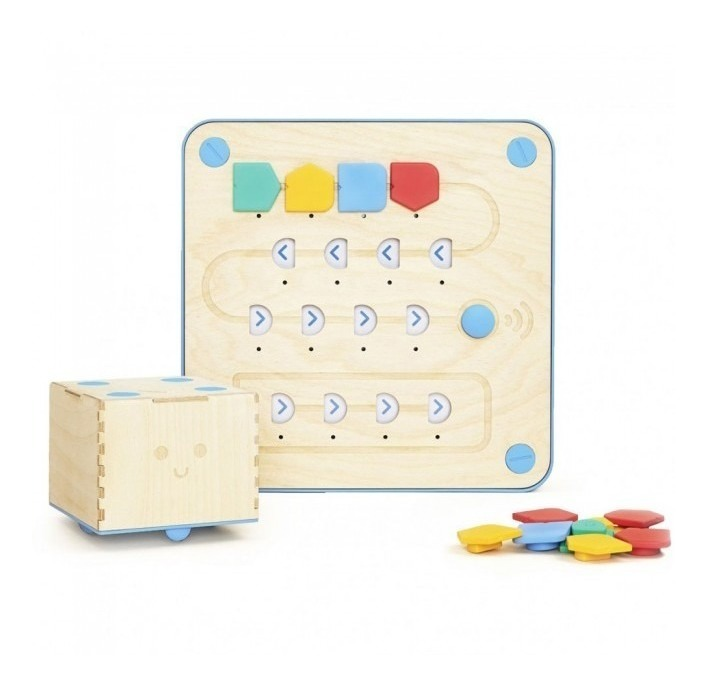
\includegraphics[width=.9\linewidth,fbox]{figs/cubetto.jpg}
        \caption{Cubetto}
        \label{fig_cubetto}
    \end{subfigure}%
    \begin{subfigure}{.5\textwidth}
        \centering
        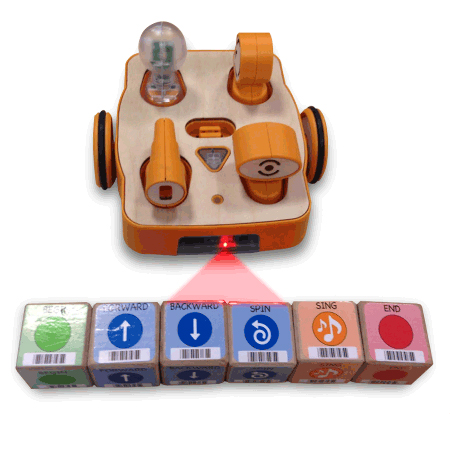
\includegraphics[width=.9\linewidth,fbox]{figs/kibo_2.jpeg}
        \caption{KIBO}
        \label{fig_kibo}
    \end{subfigure}
    \caption{Brinquedos com interfaces tangíveis.}
    \label{fig_toys_tangible}
\end{figure}

Por outro lazo, sem componentes eletrônicos, como LEDs, os blocos tangíveis carecem de meios para representar as instruções do algoritmo que durante a sua execução. A ausência de um indicador dificulta para a criança relacionar o comando está sendo executado e seus efeitos no comportamento do brinquedo. Portanto, também dificulta encontrar causas de erros, bem como mapear símbolos (imagens presente nos blocos) ações (movimentos do brinquedo).

Uma abordagem possível para diminuir a necessidade de eletrônicos também possibilitar indicadores luminosos na interface de programação é \ac{RA} projetiva \cite{roberto_dynamic_2013}. Elá é uma técnica de projeção de elementos virtuais associados a objetos reais. Ela permite que um projetor crie animações, luzes, ou qualquer objeto graficamente representável e os projete interagindo com objetos reais em uma cena. Permite, portanto, avançar a representação oferecida por LEDS fixos em blocos e painéis, ao variar as cores e formas projetadas. Deste modo, os blocos tangíveis do algoritmo podem ser construídos com materiais diversos e ainda assim proporcionar \textit{feedbacks imediatos} \cite{norman_design_1990} durante a depuração.

O RoPE (Robô Programável Educacional) representa uma oportunidade para testar a viabilidade desta abordagem de criação de interfaces tangíveis externamente compiladas e com uso de RA projetiva. Ele é um BP desenvolvido na Univali pelo Laboratório Lite\footnote{\url{https://lite.acad.univali.br}} com foco em crianças a partir dos 3 anos. A sua interface de programação são botões coloridos (\autoref{fig_rope}), desenhados para serem simples de usar por crianças pequenas \cite{raabe_2017_rope}. Essa interface se mostrou um sucesso, e o brinquedo já foi usado em Centros de Desenvolvimento Infantil por mais de 1000 crianças. Além dos botões, pesquisas desenvolveram protótipos de outros modos de interação, como um aplicativo de celular \cite{viana_cesar_interface_2018} e uma interface de programação em similar ao Cubetto \cite{metzger_desenvolvimento_2018}.

\begin{figure}[!htbp]
    \centering
    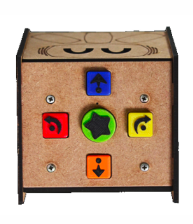
\includegraphics[width=.3\linewidth,fbox]{figs/rope_top.png}
    \caption{Brinquedo RoPE.}
    \label{fig_rope}
\end{figure}

Este trabalho ocorre como uma continuidade dessas e busca contribuir com a área de Informática na Educação ao (1) projetar uma interface tangível externamente compilada para o brinquedo RoPE e (2) explorar o uso de RA projetiva para facilitar a depuração. Essa contribuição se fundamenta na literatura sobre interfaces tangíveis para crianças \cite{sapounidis_evaluating_2015, fincher_tangible_2019, plowman_interactivity_2004} e na observação de que o uso de RA projetiva é um campo pouco explorado no contexto de BPs.

\section{Problema de Pesquisa} \label{s_cintro_problema_pesquisa}

O problema que este trabalho se propõe a investigar no contexto do brinquedo RoPE se insere no que \citeonline{norman_design_1990} denomina falta de \textit{visibilidade}. A visibilidade é um princípio de design relacionado a como o usuário percebe estado de um sistema, e como ele mapeia as ações que pode fazer e que alterações de estado elas provocam.

Em BPs que possuem apenas botões, como a Bee-Bot, o algoritmo que a criança programa não é visível. A criança não vê a sequência de comandos construída ao apertar os botões. Essa invisibilidade dificulta conversar sobre o algoritmo, analisá-lo, encontrar erros e desfazer operações. \citeonline{raabe_brinquedos_2015} menciona esse a incompreensão do funcionamento do botão de limpar a memória da Bee-Bot. As crianças esqueciam de limpar os comandos programados anteriormente, dado que essa ação não é automática. O estado do sistema não é visível, e a criança não sabe se os comandos foram limpos. A solução sugerida foi adicionar um visor de comandos.

No caso das interfaces de blocos tangíveis externamente compiladas (como a utilizada pelo KIBO), o problema é a \textit{invisibilidade de execução} do algoritmo. Os blocos carecem de indicadores que mostrem qual bloco está sendo executado em cada momento, correspondente a cada movimento do brinquedo. Essa falta de visibilidade de execução dificulta compreender a sequência lógica de funcionamento do algoritmo, pois não há mapeamento entre comando/bloco e ação do robô. O Cubetto soluciona esse problema através de luzes indicadoras, e para isso depende de um painel onde os blocos são encaixados.

\citeonline{norman_design_1990} comenta que dispositivos cujas interfaces não demonstram o estado interno durante a interação podem influenciar o entendimento do usuário sobre como tal dispositivo funciona. Esse “entendimento” é denominado modelo mental. Caso o dispositivo executar de forma inesperada, o usuário tende a encontrar alguma explicação para justificar tal comportamento. Ao justificá-lo, cria um modelo mental incorreto. \citeonline{raabe_brinquedos_2015} apresentam crianças justificando comportamentos inesperados da Bee-Bot após terem esquecido de limpar sua memória, afirmando que a “abelha” tinha vontade própria.

Por fim, essa falta de visibilidade desencadeia a dificuldade em depurar. A literatura \cite{carver_assessing_1986, mccauley_debugging_2008} apresenta modelos organizam a ação de depurar em etapas, entre as quais está a de localizar e reparação erros em algum código-fonte. A ausência do código-fonte, portanto, impede a depuração segundo estes modelos.

Partindo destas reflexões, elaborou-se a seguinte pergunta de pesquisa: 
\textit{como crianças de 4 a 6 anos interagem com uma interface de programação focada em permitir visualizar os passos e a execução de um algoritmo?}

\begin{comment}
    \begin{quadro}[!htbp]
 \caption{Vantagens e desvantagens de botões, cartas, tangíveis e aplicativos}
 \label{quadro_vantagem_desvantagem} 
 \begin{center}
 \begin{footnotesize} 
\begin{tabular}{|p{3cm}|p{3cm}|p{4.5cm}|p{4.5cm}|}
\hline
Tipo de interface & Exemplos            & Vantagens & Desvantagens\\ \hline
Botões            & RoPE, Bee-Bot       & - Facilidade de inserir comandos & - Não mostra algoritmo. \newline 
                                                                             - Não permite editar comandos, somente apagar tudo e recomeçar.
\\ \hline
Cartas            & Bee-Bot, \newline
                    Go-Robot Mouse      & - Baixo custo \newline                
                                          - Permite colaboração \newline
                                          - Customizável \newline           & - Falta de sincronia \newline 
\\ \hline
Aplicativos       & Dash, Sphero        & - Sincronia \newline 
                                          - Baixo Custo \newline
                                          - Replicabilidade \newline
                                          - Depuração \newline              & - Tempo de tela \newline
                                                                              - Difícil colaboração

\\ \hline
Blocos tangíveis  & Cubetto, KUMIITA    & - Experiência sensorial
                                          - Colaborativo \newline   
                                          - Algoritmo visível \newline      & - Custo
\\ \hline
                                        
\end{tabular}
 
 \end{footnotesize}
 \end{center} 
 \sourceauthor
\end{quadro}
\end{comment}

\subsection{Solução Proposta}
\label{ss_cintro_solucao}

A proposta é desenvolver uma interface de \ac{RA} projetiva combinada com uma linguagem externamente compilada. Dado que os blocos de linguagens externamente compiladas tem marcas fiduciais, uma câmera pode captar as posições dos blocos e um algoritmo pode controlar um projetor para destacá-los \autoref{idea}.

\begin{figure}[!htpb]
  \centering
  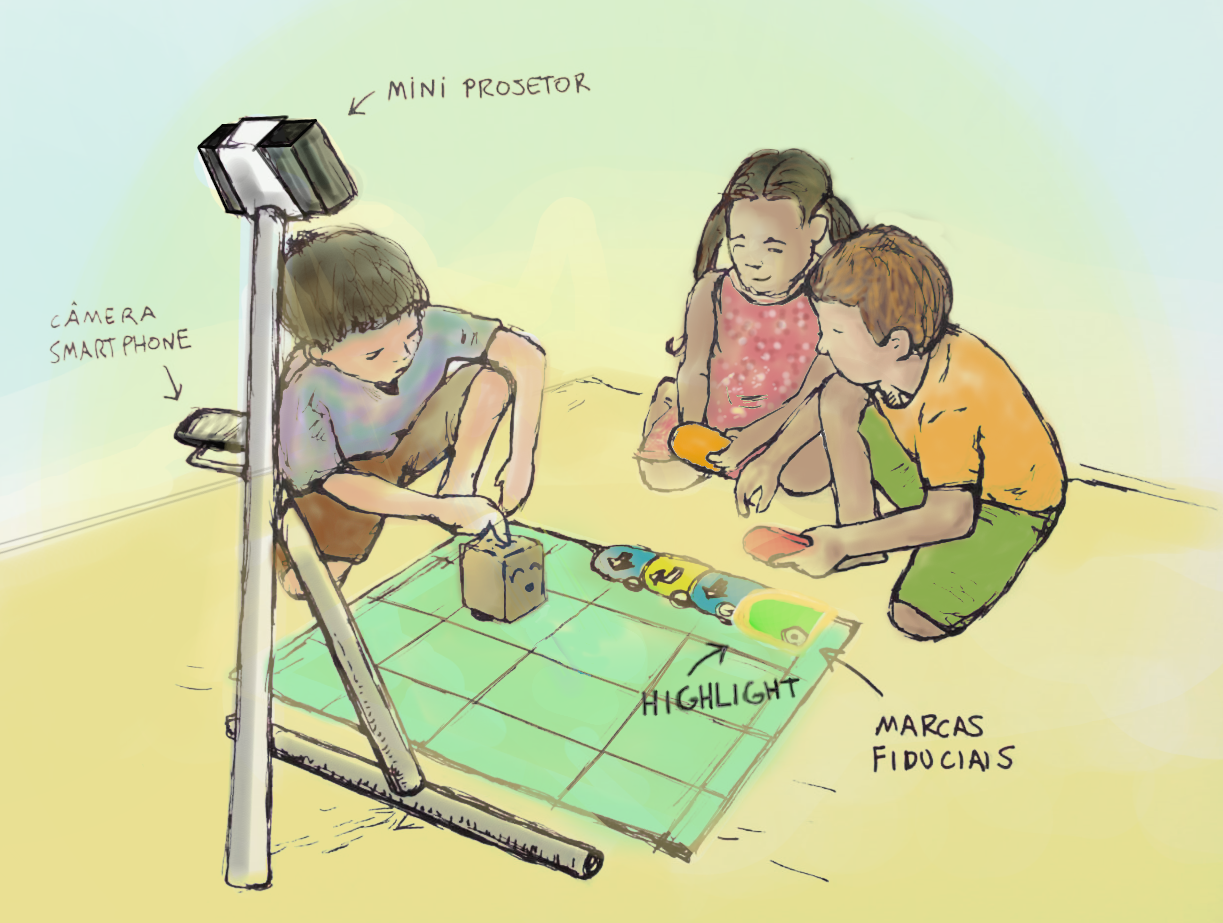
\includegraphics[width=.85\linewidth,fbox]{figs/idea_2.png}
  \caption{Solução proposta: interface tangível com realidade aumentada.}
  \sourceauthor
  \label{idea}
\end{figure}

A intenção é que a criança programe utilizando blocos de papelão com símbolos de setas correspondentes às ações do RoPE. Um \textit{smartphone} é usado como câmera, pois é mais acessível e fácil de manusear do que um notebook ou desktop. Um projetor portátil, de baixa potência de iluminação (1200 lumens) e de baixo custo ilumina os blocos e projeta um mapa interativo.

Outra funcionalidade implementada é o estado de \textit{execução passo a passo}. Ao ativar esse estado o brinquedo executa um comando e espera a criança disparar a execução da próxima ação. Isso possibilita à criança mais tempo para olhar cada bloco e compreender o movimento associado a ele. A intenção é que a criança possa compreender possíveis erros no algoritmo construído por ela ou por outra criança.

A partir do uso de RA e de um estado de execução passo a passo, a proposta é possibilitar um melhor entendimento, por parte da criança, a respeito do algoritmo que ela está construindo, e sobre seu próprio modo de pensar. Esta abordagem é exploratória, e não foram encontrados dados quantitativos passíveis de comparações numéricas com outros estudos. Este trabalho, portanto, apresenta a construção da proposta e a avaliação qualitativa das interações de crianças de 4 a 6 anos com a mesma.

\subsection{Delimitação de Escopo}
\label{ss_cintro_escopo}

Este trabalho é sobre uma ferramenta para facilitar o aprendizado de algoritmos por crianças. Algoritmos é um dos quatro pilares do \acl{PC} \cite{brackmann_desenvolvimento_2017}, junto à decomposição, abstração e reconhecimento de padrões. Este trabalho cita definições destes pilares, porém a solução proposta tem foco apenas em algoritmos, e, mais especificamente, na atividade de depurá-los.

Não é objetivo deste trabalho realizar testes com comprovação estatística, no sentido de identificar relações de causa e efeito no aprendizado. O foco é descrever a presença ou ausência das dificuldades mais perceptíveis durante a interação com uma ferramenta educacional. Esse foco se adequa à pesquisa de cunho qualitativo, com um número reduzido de crianças.

Também não foi objetivo programar um algoritmo de visão computacional para reconhecer os blocos tangíveis e o RoPE. Uma biblioteca de identificação de marcas fiduciais permitiu agilizar a implementação de um protótipo funcional. A eliminação de marcas fiduciais poderá ocorrer em trabalhos futuros, considerando os aprendizados obtidos com a primeira versão aqui apresentada.

% ----------------------------------------------------------------------- %
\subsection{Justificativa}
\label{ss_cintro_justificativa}

O mapeamento industrial descrito no \autoref{c_estado_arte}, demonstra que, de 56 brinquedos, apenas 2 utilizam RA. Ainda assim o seu uso ocorre através de tablets e celulares, menos indicados para crianças em comparação com as interfaces tangíveis \cite{sapounidis_tangible_2019, zuckerman_tui_2013}.

No mesmo mapeamento, o RoPE aparece como o único projeto brasileiro em atividade voltado ao ensino de programação para crianças pequenas com brinquedos programáveis. Desde a sua concepção, o projeto estuda aspectos de design para que crianças possam aprender de forma lúdica e evitando erros não construtivos \cite{raabe_brinquedos_2015}. A abordagem aplicando \ac{RA}, como este trabalho propõe, ainda não foi experimentado com o RoPE ou outros brinquedos. Considerando o pioneirismo do RoPE como ferramenta educacional para aprendizado de algoritmos por crianças no Brasil, entende-se que a exploração proposta neste trabalho pode contribuir com novas informações para o projeto.

A reprodução da proposta é facilitada pelo fato da mesma não utilizar componentes eletrônicos específicos. Os componentes usados são produtos disponíveis comercialmente, que precisam ser plugados (mini-projetores, \textit{smartphones} e Arduino). O RoPE compartilha princípio de ser programado por botões com diversos outros brinquedos, como a Bee-Bot, Go Robot Mouse e Thymio. Esses brinquedos também poderiam ser aplicados no contexto da proposta, o que também facilita sua reprodução.

A proposta de usar \ac{RA} projetiva abre caminho para desenvolver tapetes dinâmicos. Atualmente o brinquedo RoPE se move sobre tapetes estáticos, que precisam ser trocados conforme a atividade. A projeção, associado à informação da localização do brinquedo, permite disparar eventos quando este atinge determinadas posições. Esses eventos viabilizam a construção de jogos, em que as fases avançam conforme os movimentos do brinquedo. Portanto, ao permitir que um sistema computacional perceba a posição do brinquedo e projete o ambiente, surgem novas possibilidades de interação.

Novas possibilidades de interação também surgem ao utilizar a programação em blocos. Por estarem desassociados dos botões do RoPE, os blocos podem expandir as funções já existentes sem a necessidade de modificações físicas no brinquedo. Enquanto os botões definem ações específicas, como giros de 90.º, adequadas para as crianças iniciarem os primeiros algoritmos, os blocos podem definir outros movimentos, como giros de 45.º, por exemplo. Além disso, outros blocos podem programar eventos de sons e luzes, e também animações como trocar o mapa projetado.

Entretanto, prosseguir com essas possibilidades exige avaliar a ferramenta no em centros de desenvolvimento infantil com crianças de 4 a 6 anos. Essa avaliação é necessária por dois motivos principais. Primeiro, obter a opinião de professores e crianças sobre a interface; e segundo, verificar riscos, como a criança obstruir as marcas fiduciais, ou os elementos físicos e virtuais representarem uma fonte de distração e não de aprendizado.

Por fim, a proposta está ligada a uma área de interesse da comunidade científica\footnote{Possui jornais dedicados ao tema, como International Journal of Child-Computer Interaction e ACM Transactions on Computer-Human Interaction.}, e ao fato de que há uma lacuna de compreensão sobre utilização de \ac{RA} projetiva com brinquedos programáveis.

\section{Objetivos}
\label{s_cintro_objetivos}

\subsection{Objetivo Geral}
\label{ss_cintro_objetivo_geral}

Avaliar qualitativamente o uso de uma interface de \ac{RA} projetiva na depuração de algoritmos do brinquedo RoPE por crianças de 4 a 6 anos.

\subsection{Objetivos Específicos}
\label{ss_cintro_objetivos_espec}

Os objetivos específicos do trabalho são:

\begin{enumerate}
    
    \item Relacionar sistemas e aplicações que utilizam realidade aumentada projetiva;

    \item\label{obj_mapear} Categorizar as interfaces de brinquedos programáveis existentes;

    \item\label{obj_interface} Construir a interface de realidade aumentada projetiva para o brinquedo RoPE;

    \item\label{obj_avaliar} Aplicar a interface em atividades com crianças para coletar e analisar eventos de interação.
    
\end{enumerate}
\section{Metodologia}
\label{s_cintro_metodologia}

Esta seção descreve a metodologia e os procedimentos metodológicos utilizados nesta pesquisa.

\subsection{Métodos da Pesquisa}
\label{ss_cintro_metod_pesquisa}

Métodos científicos são conjuntos de procedimentos técnicos adotados para produzir conhecimento \cite{gil_metodos_2008}, construído através de passos para atingir os objetivos de uma pesquisa \cite{wazlawick_metodologia_2009}. O método desta pesquisa pode ser descrito como de natureza aplicada, pois prevê a aplicação prática de uma ferramenta e tecnologias para solucionar um problema de interação com brinquedos programáveis. A abordagem sobre o problema foi qualitativa, ao observar aspectos subjetivos como falas, gestos e expressões durante o uso da solução proposta. Por fim, esta pesquisa é exploratória, ao buscar extrair informações de um fenômeno desconhecido, a partir de uma pequena amostra de participantes em caráter experimental. A próxima subseção descreve os procedimentos metodológicos adotados.

\subsection{Procedimentos Metodológicos}
\label{ss_cintro_proced_metodologicos}

A construção da solução proposta e atendimento dos objetivos de pesquisa possui quatro fases: estudo, modelagem, implementação e avaliação, descritas a seguir.

\begin{description}
    \item[Estudo] Essa etapa correspondeu a uma revisão sistemática, um mapeamento industrial e um levantamento de trabalhos similares. A revisão sistemática focou em compreender como são feitas pesquisas científicas avaliando interfaces de programação de brinquedos programáveis. O mapeamento buscou descrever as categorias de interfaces mais utilizados em projetos de brinquedos programáveis, incluindo produtos comerciais. Por último, trabalhos similares descrevem o uso de projeção ou formas de facilitar a programação por crianças.

    \item[Modelagem] A etapa de modelagem ocorreu como um planejamento dos elementos de software a serem implementados. Esta etapa envolveu levantamento de requisitos (\autoref{apendice_requisitos}) e prototipação (\autoref{apendice_prototipo}) para conferir a viabilidade da proposta. 

    \item[Implementação] Etapa que correspondeu a programar o aplicativo (i) alterar o \textit{firmware} do brinquedo RoPE para comunicação sem fio; (ii) configurar a conexão com uma plataforma de armazenamento das interações ocorridas com um brinquedo programável; (ii) adaptar o \textit{firmware} do RoPE para comunicação sem fio; e (iii) programar um aplicativo de \textit{smartphone} para captar os blocos e comunicar com o projetor.
   
    \item[Avaliação] A avaliação\footnote{Para atendimento do objetivo específico \autoref{obj_avaliar}.} aqui compreendida na observação de crianças em atividades de programação do RoPE, para coletar e por fim analisar dados seguindo um protocolo definido no \autoref{c_avaliacao}. Essa etapa envolveu aplicação do software de  análise qualitativa Qualcoder, para tratamento dos dados coletados. 

\end{description} 

\section{Estrutura da Dissertação}
\label{s_cintro_estrutura}

O trabalho está organizado em 6 capítulos correlacionados. O \autoref{c_introducao}, contextualizou e apresentou o tema, o problema e uma proposta de como solucioná-lo. Foram estabelecidos os objetivos a serem alcançados com a solução, e as limitações de escopo a serem observadas.

O \autoref{c_fundamentacao_teorica} apresenta a fundamentação teórica iniciando com a descrição do sujeito desta pesquisa (a criança) e observa fundamentos relacionados ao desenvolvimento infantil. Como tema relacionado a algoritmos, é apresentada a definição de \ac{PC} em quatro pilares. O capítulo também apresenta fundamentos sobre as interfaces de brinquedos programáveis, bem como aplicações de realidade aumentada projetiva.

O \autoref{c_estado_arte} apresenta o estado da arte em três aspectos: das pesquisas realizadas com brinquedos programáveis; interfaces de brinquedos mais utilizados no mercado; e trabalhos com semelhanças tecnológicas e conceituais.

\autoref{c_desenvolvimento} é o quarto capítulo, que apresenta uma visão geral dos componentes da contribuição: aplicativo e elementos tangíveis. O capítulo apresenta aspectos técnicos da implementação, tecnologias utilizadas para construir esses componentes e possibilitar a comunicação entre os mesmos.

O \autoref{c_avaliacao} descreve o contexto de execução da pesquisa. Ele também apresenta o protocolo de teste e os instrumentos de coleta usados durante atividades com crianças. Em seguida, o \autoref{c_resultados} apresenta os resultados obtidos com a análise dos dados coletados.

Por fim, o \autoref{c_conclusao} revisa o atendimento aos objetivos da pesquisa, reflete sobre as contribuições geradas e propõe trabalhos futuros.